\documentclass[14pt]{extarticle}

\usepackage[utf8]{inputenc}
\usepackage[T2A]{fontenc}
\usepackage[russian]{babel}

\usepackage[a4paper,margin=2.5cm]{geometry}

\usepackage{amsmath}
\usepackage{amssymb}
\usepackage{amsthm}
\usepackage{mathrsfs}
\usepackage{enumitem}
\usepackage{titlesec}

\usepackage{graphicx}
\usepackage{float}

\usepackage[notlof,notlot]{tocbibind}
\usepackage{needspace}

\usepackage{hyperref}
\usepackage{cleveref}

\titlespacing{\subsection}{0pt}{4\baselineskip}{1\baselineskip}
\titlespacing{\subsubsection}{0pt}{2\baselineskip}{1\baselineskip}

\setlist[enumerate]{noitemsep, topsep=0pt}

\setcounter{secnumdepth}{3}
\setcounter{tocdepth}{3}

\newtheoremstyle{breakstyle}  % Имя стиля
  {\topsep}                   % Отступ сверху
  {\topsep}                   % Отступ снизу
  {\normalfont}               % Шрифт для тела
  {0pt}                       % Отступ для тела
  {\bfseries}                 % Стиль заголовка
  {.}                         % Знак после заголовка
  {\newline}                  % Пространство после заголовка: новая строка
  {}                          % Спецификация заголовка

\theoremstyle{breakstyle}
\newtheorem{definition}{Определение}[subsection]
\newtheorem{theorem}{Теорема}[subsection]
\newtheorem{lemma}{Лемма}[subsection]

\setlength{\parindent}{0pt} 

\title{ТВиМС-2025}

\begin{document}
\maketitle

\tableofcontents

\clearpage
\section{Теория вероятностей.}

\subsection{Основы теории вероятностей и схема Бернулли.}

\subsubsection{Классическое и геометрическое определение вероятности.}
\begin{definition}[Пространство элементарных событий]

$\Omega$ - пространство элементарных событий. \\
$\omega_1$, $\omega_2$, ... - элементарные события. \\
$A \subset \Omega$ - случайное событие.
$\mathscr{A} = \{A \subset \Omega\}$ - $\sigma$-алгебра подмножеств.

\end{definition}

\begin{definition}[$\sigma$-алгебра событий]

Свойства алгебры событий:
\begin{enumerate}
    \item $\Omega \in \mathscr{A}$ - достоверное событие.
    \item Если $A \subset \mathscr{A}$, то $\overline{A} \subset \mathscr{A}$
    \item $\emptyset$ - невозможное событие.
    \item Если A, B - события (т.е. принадлежат $\mathscr{A}$), то $A \cup B$ и $A \cap B$ - события. 
\end{enumerate}

\vspace{\baselineskip}
Свойства $\sigma$-алгебра событий:
\begin{enumerate}
    \item Все свойства алгебры событий.
    \item Если $A_1$, $A_2$, ... , $A_n \in \mathscr{A}$, то:
    \begin{enumerate}
        \item $\bigcup_{i=1}^{\infty} A_i \in \mathscr{A}$
        \item $\bigcap_{i=1}^{\infty} A_i \in \mathscr{A}$
    \end{enumerate}
\end{enumerate}

\vspace{\baselineskip}

\textbf{Алгебра событий} - семейство подмножеств $\Omega$, замкнутое относительно операций конечного объединения, пересечения и дополнения. \\
\textbf{$\sigma$-алгебра событий} - семейство подмножеств $\Omega$, замкнутое относительно операций счетного объединения, пересечения и дополнения.

\vspace{\baselineskip}

\textbf{Минимальная $\sigma$-алгебра} - это $\sigma$-алгебра, из которой при убирании одного любого элемента, пересатет быть $\sigma$-алгеброй.

\end{definition}

\begin{figure}[H]
    \centering
    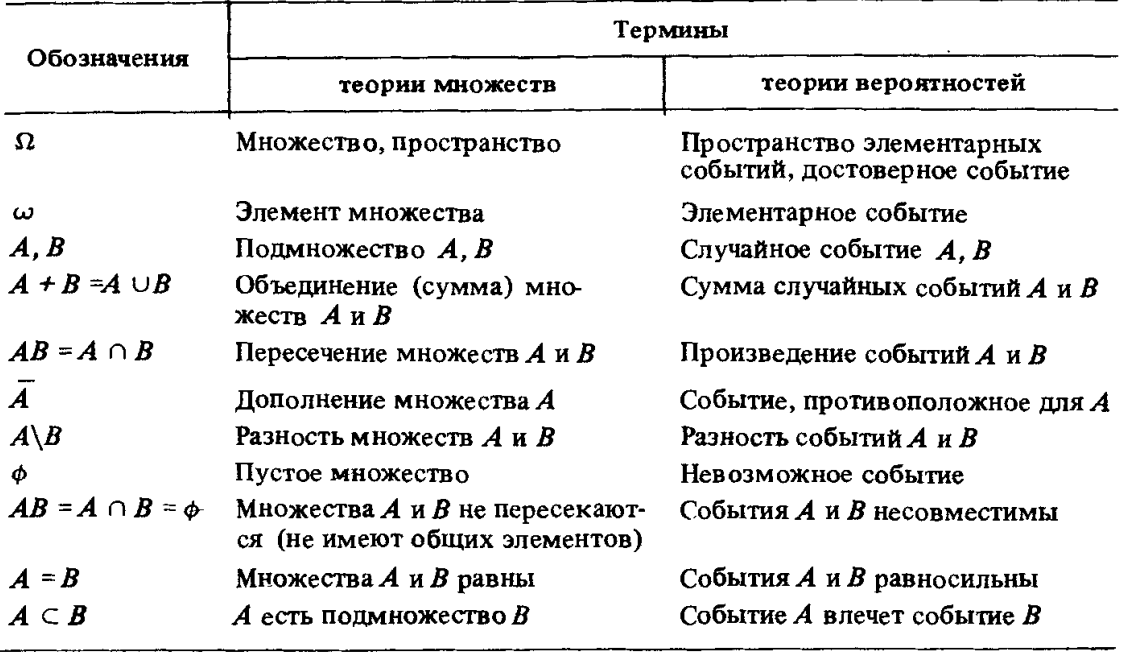
\includegraphics[width=0.7\textwidth]{images/table.png}
    \caption{Таблица соответствий}
    \label{fig:prob-table}
\end{figure}

\begin{definition}[Класическое определение вероятности]

Пусть $\mid \Omega \mid = n$
$P(\omega_i) = \frac{1}{n}$ (т.е. события равновероятны). \\
$A \subset \Omega$ - событие (подмножество элементарных событий). \\
$\mid A \mid = k \rightarrow P(A) = \frac{k}{n}$ \\
Следовательно, $0 \leq P(A) \leq 1$.

\end{definition}

\begin{definition}[Геометрическое определение вероятности]

Рассматриваем Лебегову $\sigma$-алгебру $\rightarrow$ mes (мера) - существует и конечна. \\
\textbf{Мера Лебега} - мера, обобщающая понятия длины отрезка, площади фигуры и объёма тела на произвольное n-мерное евклидово пространство. \\

$0 < mes(\Omega) < +\infty$ \\
$mes(\omega_i) = 0$ \\
$A \subset \Omega \rightarrow P(A) = \frac{mes(A)}{mes(\Omega)}$

\vspace{\baselineskip}
Проще говоря:
$\Omega$ - плоское, значит у $\Omega$ $\exists$ площадь, и она конечна. \\
$0 < S(\Omega) < +\infty$ \\
$S(\omega_i) = 0$\\
$A \subset \Omega \rightarrow P(A) = \frac{S(A)}{S(\Omega)}$ \\

\end{definition}

\subsubsection{Основные комбинаторные формулы.}
\begin{definition}[Размещения]
\textbf{Размещения} - способ расположить в определенном порядке некоторого числа элементов из заданного конечного множества.

\vspace{\baselineskip}

\textbf{Формулы:}
\begin{enumerate}
    \item \textbf{Размещения без повторений:} $A_{n}^{k} = n(n-1)(n-2)...(n-k+1) = \frac{n!}{(n - k)!}$
    \item \textbf{Размещения с повторениями:} $U_{n}^{k} = n \cdot n \cdot ... \cdot n = {n}^{k}$
\end{enumerate}    

\end{definition}

\begin{definition}[Сочетания]
\textbf{Сочетания} - способ расположения с несущественной последовательностью выбора некоторого числа элементов из заданного конечного множества.

\vspace{\baselineskip}

\textbf{Формулы:}
\begin{enumerate}
    \item \textbf{Сочетания без повторений:} $C_{n}^{k} = \frac{A_{n}^{k}}{k!} = \frac{n!}{(n - k)! \cdot k!}$
    \item \textbf{Сочетания с повторениями:} $V_{n}^{k} = C_{n+k-1}^{n-1} = \frac{(n+k-1)!}{k! \cdot (n-1)!}$
\end{enumerate} 

\end{definition}

\subsubsection{Аксиоматика Колмогорова.}
\begin{definition}[Несовместные события]

События A и B - несовместные $\leftrightarrow$ $A \cap B = AB = 0$. \\
Т.е. события не могут наступить одновременно.

\end{definition}

\begin{definition}[Вероятность как функция]
$\Omega$ - пространство элементарных событий. \\
$\omega_i \in \Omega$ - элементарное событие. \\
$\mathscr{A}$ - $\sigma$-алгебра событий. \\

Тогда вероятность P - функция на множестве событий:
$P: \mathscr{A} \rightarrow [0; 1]$ \\

Со следующими \textbf{аксиомами:}
\begin{enumerate}
    \item $P(\Omega) = 1$
    \item $\forall A, B: A \cap B = \emptyset \rightarrow P(A \cup B) = P(A) + P(B)$
    \item (Счетная аддитивность) $\forall A_1, ... , A_n \in \mathscr{A}$ $P(\bigcup_{i=1}^{\infty} A_i) = \Sigma_{i=1}^{\infty}P(A_i)$, причем $A_{i}A_{j} = \emptyset$, если $i \neq j$
\end{enumerate}

\vspace{\baselineskip}

Из аксиом можно получить данные \textbf{следствия:}
\begin{enumerate}
    \item $P(\emptyset) = 0$
    \item $P(\overline{A}) = 1 - P(A)$
    \item $A \subset B \rightarrow P(A) \leq P(B)$
\end{enumerate}

\end{definition}

\subsubsection{Условная вероятность. Независимость. Формулы сложения и умножения.}
\begin{definition}[Условная вероятность]

A, B - события, причем: $P(A) > 0$. \\
Тогда вероятность события B при \textbf{условии} A: \\
$P(B | A) = \frac{P(AB)}{P(A)} = P_{A}(B)$

\end{definition}

\begin{definition}[Формула умножения]
A, B - события: $P(A) > 0$ и $P(B) > 0$. \\
\textbf{Формула умножения:} $P(AB) = P(B | A) \cdot P(A) = P(A | B) \cdot P(B)$ \\

\textbf{Пример:} \\
В колоде 36 карт. На удачу вытащили 2 карты. Какова вероятность, что обе карты - пики?\\

\begin{enumerate}
    \item \textbf{Класическая вероятность:} $\frac{Число благоприятных исходов}{Общее число исходов} = \frac{C_{9}^{2}}{C_{36}^{2}} = \frac{9 \cdot 8}{36 \cdot 35}$
    \item \textbf{Формула умножения:} A - первая карта - пики, B - вторая карта - пики. Тогда $P(AB) = P(A) \cdot P(B | A) = \frac{9}{36} \cdot  \frac{8}{35}$
\end{enumerate}

\end{definition}

\begin{theorem}[Условная вероятность и аксиоматика Колмогорова]

Зафиксируем $A \subset \Omega$: $P(A) \neq 0$. \\
Тогда $P_{A}(B)$ - подчиняется аксиоматике Колмогорова, т.е. для нее выполняются те же аксиомы.

$\square$

\textbf{Доказательство 1ой аксиомы:} \\
$P_{A}(\Omega) = \frac{P(\Omega A)}{P(A)}$ \\
Т.к. $A \subset \Omega$, то $\Omega A = A$ \\
Следовательно, $P_{A}(\Omega) = \frac{P(A)}{P(A)} = 1$ \\

\textbf{Доказательство 2ой аксиомы:} \\
Пусть B, C - события: $BC = \emptyset$, тогда: \\
$P_{A}(B \cup C) = \frac{P(A(B \cup C))}{P(A)} = \frac{P(AB \cup AC)}{P(A)}$ \\
Т.к. $BC = \emptyset$, получаем: $ABAC = ABC = \emptyset$, т.е. события $AB$ и $AC$ - несовместны. \\
Следовательно, $\frac{P(AB \cup AC)}{P(A)} = \frac{P(AB) + P(AC)}{P(A)}$ \\
Значит, $P_{A}(B \cup C) = \frac{P(AB) + P(AC)}{P(A)}$ \\

\vspace{\baselineskip}

$P_{A}(B) = \frac{P(AB)}{P(A)}$ \\
$P_{A}(C) = \frac{P(AC)}{P(A)}$ \\
Значит, $P_{A}(B) + P_{A}(C) = \frac{P(AB) + P(AC)}{P(A)}$ \\

\vspace{\baselineskip}

Итог: $P_{A}(B \cup C) = \frac{P(AB) + P(AC)}{P(A)} = P_{A}(B) + P_{A}(C)$ \\

\textbf{3яя аксиома} доказывается аналогичным образом.

\hfill$\blacksquare$

\end{theorem}

\begin{definition}[Независимые события. Попарно независимые события. Независимые в совокупности события]

Пусть A и B - события. \\
Тогда A и B называют \textbf{независимыми событиями} $\leftrightarrow$ $P(AB) = P(A) \cdot P(B)$ \\

Пусть $A_{1}, ... , A_{n}$ - события. \\
Тогда они \textbf{попарно независимы}, если $\forall i \neq j$, $A_{i}$ и $A_{j}$ независимы. \\

Пусть $A_{1}, ... , A_{n}$ - события. \\
Тогда они \textbf{независимы в совокупности}, если $\forall k \in \overline{[2..n]}$ и $\forall$ набора $1 \leq i_{1} < i_{2} < ... < i_{k} \leq n$, выполняется: $P(A_{i_{1}}A_{i_{2}}...A_{i_k}) = P(A_{i_{1}})P(A_{i_{2}})...P(A_{i_{k}})$

\end{definition}

\begin{definition}[Формула сложения]

Пусть A, B - события, тогда: \\
$P(A \cup B) = P(A) + P(B) - P(AB)$

$\square$

$P(A \cup B) = P(A \overline{B} \cup AB \cup B \overline{A}) = P(A \overline{B}) + P(AB) + P(B \overline{A})$ \\

\vspace{\baselineskip}

$A = A \Omega = A(\overline{B} \cup B) =  A \overline{B} \cup AB$ \\
$B = AB \cup B \overline{A}$ \\

\vspace{\baselineskip}

$P(A \cup B) = P(A \overline{B}) + P(AB) + P(B \overline{A}) + P(BA) - P(AB) = P(A) + P(B) - P(AB)$ \\
Итог: $P(A \cup B) = P(A) + P(B) - P(AB)$ \\

\hfill$\blacksquare$

\vspace{1\baselineskip}

Пусть A, B, C - события. \\
Аналогично (через разбиения на несовместные), доказывается следующее: \\
$P(A \cup B \cup C) = P(A) + P(B) + P(C) - P(AB) - P(BC) - P(AC)$ \\

\vspace{\baselineskip}

Формула сложения в \textbf{общем виде:}\\
$A_{1}, ... , A_{n}$ - события.

$P(A_{1} \cup ... \cup A_{n}) = \Sigma_{i=1}^{n}P(A_{i}) + ... + {(-1)}^{r+1}\Sigma_{1 \leq i_{1} < i_{2} < ... < i_{r} \leq n}P(A_{i_{1}}A_{i_{2}}...A_{i_{r}}) + ... + {(-1)}^{n}P(\bigcap_{i=1}^{n}A_{i})$ \\

\vspace{\baselineskip}
Если, дополнительно, $A_{1}, ... , A_{n}$ - независимы в совокупности, то: \\
$P(\bigcup_{i=1}^{n}A_{i}) = 1 - P(\bigcap_{i=1}^{n}\overline{A_{i}}) = 1 - \sqcap_{i=1}^{n}(1 - P(A_{i}))$

\end{definition}

\subsubsection{Формула полной вероятности.}
\begin{definition}[Формула полной вероятности]

Разобъем множество элементарных событий $\Omega$ на независимые попарно гипотезы $H_{1} ... H_{n}$. \\
Т.е. $\Omega = \bigcup_{i=1}^{n}H_{i}$ и $\forall i \neq j \rightarrow H_{i}H_{j} = \emptyset$. \\
Причем $\forall i H_{i} > 0$, иначе объединим эту гипотизу с другой. \\

\vspace{\baselineskip}

\textbf{Формула полной вероятности:} $P(A) = \Sigma_{i=1}^{n}P(A | H_{i})P(H_{i})$

$\square$

$\forall A \in \mathscr{A} \rightarrow P(A) = P(A \Omega) = \bigcup_{i=1}^{n}(AH_{i})$ \\
По попарной независимости и правилу умножения: $\bigcup_{i=1}^{n}(AH_{i}) = \Sigma_{i=1}^{n}(AH_{i}) = \Sigma_{i=1}^{n}P(A | H_{i})P(H_{i})$ \\

\hfill$\blacksquare$

\end{definition}

\subsubsection{Формула Байеса.}
\begin{definition}[Формула Байеса]

Для получения вероятности наступления конкретной гипотезы используется формула Байеса. \\

A - событие: $P(A) \neq 0$, $H_{1}, ... , H_{i}$ - гипотезы, тогда: \\
\textbf{Формула Байеса:} $P(H_{i} | A) = \frac{P(A | H_{i}) \cdot P(H_{i})}{P(A)} = \frac{P(A | H_{i}) \cdot P(H_{i})}{\Sigma_{j=1}^{n}P(A | H_{j}) \cdot P(H_{j})}$

\end{definition}

\subsubsection{Испытания Бернулли. Формула Бернулли.}
\begin{definition}[Испытания Бернулли]

\textbf{Испытания Бернулли} - последовательность независимых испытаний с бинарным исходом. \\

Пространство элементарных событий - набор двоичных слов. Например: \\
Подбрасываются 3 монеты: 0 - решка (неудача), 1 - орел (успех). $P$(выпал орел) $= p$ и $P$(выпала решка) $= q$.\\

События: \\
0 0 0 (вероятность - $q^{3}$)\\
0 0 1 (вероятность - $p \cdot q^{2}$)\\
0 1 0 (вероятность - $p \cdot q^{2}$)\\
0 1 1 (вероятность - $p^{2} \cdot q$)\\
1 0 0 (вероятность - $p \cdot q^{2}$)\\
1 0 1 (вероятность - $p^{2} \cdot q$)\\
1 1 0 (вероятность - $p^{2} \cdot q$)\\
1 1 1 (вероятность - $p^{3}$)\\

Введем дополнительные обозначения: \\
Пусть $S_{n}$ - число успехов в $n$-испытаниях Бернулли, тогда: \\
$P(S_{n} = k) := P_{n}(k)$, $\forall k \in \overline{[0..n]}$ \\
$P(m_{1} \leq S_{n} \leq m_{2}) = \Sigma_{k=m_{1}}^{k=m_{2}}P_{n}(k)$ $\forall$ $m_{1} \geq 0$, $m_{2} \leq n$, $m_{1} \leq m_{2}$ \\

Тогда легко можно получить \textbf{формулу Бернулли:} 
\begin{enumerate}
    \item \textbf{Для точного числа успехов:} $P_{n}(k) = C_{n}^{k}p^{k}q^{n-k}$
    \item \textbf{Для промежутка:} $P(m_{1} \leq S_{n} \leq m_{2}) = \Sigma_{k=m_{1}}^{m_{2}}C_{n}^{k}p^{k}q^{n-k}$
\end{enumerate}

\end{definition}

\begin{lemma}[Наиболее вероятное число успехов]

Число успехов, что наиболее вероятны, ограничено значением $p(n+1) - 1$. Причем для целого $p(n+1) - 1$ существует два таких числа, а для нецелого - одно. \\

$\square$

Пусть даны $n$ и $p$. Найдем $k$, при котором $P(S_{n} = k)$ - максимальное. \\
Сравним $P_{n}(k)$ и $P_{n}(k+1)$: \\

$\frac{C_{n}^{k+1}p^{k+1}q^{n-k-1}}{C_{n}^{k}p^{k}q^{n-k}} = \frac{\frac{n!}{(k+1)!(n-k-1)!} \cdot p}{\frac{n!}{k!(n-k!)} \cdot q} = \frac{n-k}{k+1} \cdot \frac{p}{1-p}$ \\
Найдем решение неравенства: $\frac{n-k}{k+1} \cdot \frac{p}{1-p} \geq 1$ \\
$(n-k)p \geq (k+1)(1-p)$ \\
$pn - pk \geq k - kp + 1 - p$ \\
$k \leq pn + p - 1$ \\
$k \leq p(n+1) - 1$ \\

Т.к. значения $p$ и $n$ даны, то можно подсчитать значение для k - наиболее вероятного числа успехов.

Рассмотрим два варианта:
\begin{enumerate}
    \item $p(n+1) - 1 \in \mathbb{Z}$: два наиболее вероятных числа успехов - $k$ и $k+1$.
    \item $p(n+1) - 1 \notin \mathbb{Z}$: одно наиболее вероятное значение.
\end{enumerate}

\hfill$\blacksquare$

\end{lemma}

\subsubsection{Пуассоновское приближение для схемы Бернулли.}
\begin{definition}[Пауссоновское приближение]
При фиксированном числе успехов и $n \rightarrow \infty$, верно следующее: \\
$C_{n}^{k}p^{k}q^{n-k} \rightarrow \frac{\lambda^{k} \cdot e^{-\lambda}}{k!}$

\end{definition}

\subsubsection{Локальная теорема Муавра – Лапласа.}
\begin{theorem}[Локальная теорема Муавра-Лапласа]

Пусть: 
\begin{enumerate}
    \item $x_{n} = \frac{k-np}{\sqrt{npq}}$: $n, k \rightarrow \infty$, $x_{n}$ - ограничено.
    \item $\phi(x) = \frac{1}{\sqrt{2\Pi}} \cdot e^{-\frac{x^{2}}{2}}$ - функция Гаусса.
\end{enumerate}

Тогда:\\
$P_{n}(k) \sim \frac{1}{\sqrt{npq}} \cdot \phi(x_{n})$, при $n \rightarrow \infty$

$\square$

\begin{enumerate}
    \item Пользуемся формулой Стирлинга: $n! \sim e^{-n}n^{n}\sqrt{2\Pi n}$.
    \item Пользуемся разложением в ряд Тейлора: $ln(1+x) = x - \frac{x^{2}}{2} + \frac{x^3}{3} + ... + (-1)^{n+1} \frac{x^{n}}{n} + o(x^{n})$
\end{enumerate}

Аккуратно расписываем $C_{n}^{k}p^{n}q^{n-k}$. При переходе от факториала к экспоненте необходимо будет прологарифмировать. \\

\hfill$\blacksquare$

\end{theorem}

\subsubsection{Интегральная теорема Муавра – Лапласа.}
\begin{theorem}[Интегральная теорема Муавра-Лапласа]

Пусть: 
\begin{enumerate}
    \item $x_{n}^{'} = \frac{k_{1}-np}{\sqrt{npq}}$: $n \rightarrow \infty$, $k_{1}$ - левая граница интервала.
    \item $x_{n}^{''} = \frac{k_{2}-np}{\sqrt{npq}}$: $n \rightarrow \infty$, $k_{2}$ - правая граница интервала.
    \item $\Phi(x) = \frac{1}{\sqrt{2\Pi}} \cdot \int_{0}^{x} e^{-\frac{x^{2}}{2}} \, dx$.
\end{enumerate}

Тогда:
$P_{n}(k_{1}; k_{2}) = \Phi(x^{''}) - \Phi(x^{'})$

\end{theorem}

\subsection{Случайные величины и их распределения.}

\subsubsection{Случайная величина. Функция распределения случайной величины, ее свойства.}
\begin{definition}[Борелевские множество и -$\sigma$-алгебра]

\textbf{Борелевское множество относительно $\mathbb{R}^{n}$} - элемент $\mathscr{B(\mathbb{R}^{n})}$ (борелевской $\sigma$-алгебры относительно $\mathbb{R}^{n}$).\\

\textbf{Борелевская $\sigma$-алгебра относительно $\mathbb{R^{n}}$} - это система множеств, которое:
\begin{enumerate}
    \item Содержит все открытые подмножества $\mathbb{R}^{n}$ (параллелепипед в общем случае; интервал для $\mathbb{R}$).
    \item Замкнута относительно операций счетного объединения, пересечения и дополнения: точки, конкретные параллелепипеды, полуплоскости ... (обычное свойство $\sigma$-алгебры). 
    \item Является минимальной $\sigma$-алгеброй: если выкинуть хотя бы один элемент из данного множества, то оно перестает быть $\sigma$-алгеброй.
\end{enumerate}

\end{definition}

\begin{definition}[Случайная величина]
\textbf{Случайная величина} $\xi$ - есть измеримая функция: $\Omega \rightarrow \mathbb{R}$. \\
$\xi = \xi(\omega)$, $\forall \omega \in \Omega$. \\
Значит, $\forall c \in \mathbb{R}$ $\rightarrow$ $P\{\xi \neq c\} = 0$ или, что $P\{\xi = c\} = 1$.

\vspace{\baselineskip}

$\xi = \xi(\omega)$ - \textbf{случайная величина}, если функция $\xi(\omega)$ измерима относительно введенной в рассматриваемом множестве $\Omega$ вероятности.

\vspace{\baselineskip}

Иначе говоря, мы требуем, чтобы для каждого измеримого по Борелю множества (т.е. являющееся Борелевским множеством) $A_{\xi}$ значений $\xi$ множество $A_{\omega}$ тех $\omega$, для которых $\xi(\omega) \subset A_{\xi}$ принадлежало множеству $\mathscr{A}$ случайных событий и, следовательно, для него была бы определена вероятность: $P\{\xi \subset A_{\xi}\} = P\{A_{\omega}\}$.

\vspace{\baselineskip}

Т.е. если для любого борелевского множества $A_\xi$ прообраз $A_\omega \in \mathscr{A}$ $\rightarrow$ $\xi$ является случайной величиной. \\
Если существует хотя бы одно борелевское множество $A_\xi$, для которого $A_\omega \notin \mathscr{A}$ $\rightarrow$ $\xi$ не является случайной величиной.

\vspace{\baselineskip}

В частности, если множество $A_{\xi}$ совпадает с полупрямой $\xi < x$, то вероятность $P\{A_{\omega}\}$ есть функция распределения переменного $x$:
$P\{\xi < x\} = P\{A_{\omega}\} = F(x)$ - функция распределения случайной величины $\xi$. \\

\vspace{\baselineskip}

Максимально \textbf{неформальное определение:}\\
\textbf{Случайная величина} - величина, значения которой зависят от случая и для которой определена функция распределения вероятностей. \\

\textbf{Примеры:}
\begin{enumerate}
    \item Константа: $\forall \omega$ $\xi(\omega) = a \in \mathbb{R}$
    \item Монета: орел +1, решка -1 \\
          $\mathscr{A} = \{\emptyset, \text{О}, \text{Р}, \Omega\}$ \\
          $\xi(\text{О}) = 1$, $\xi(\text{Р}) = -1$, $\Omega = \{\text{О}, \text{Р}\}$ \\
          $P(\xi = 1) = \frac{1}{2}$, $P(\xi = -1) = \frac{1}{2}$
    \item Число успехов в испытаниях Бернулли: $\omega \in \Omega$ - наборы длины $n$ из $0$ и $1$.
    \item Ошибки измерений.
    \item Срок службы прибора.
\end{enumerate}

\vspace{\baselineskip}

Если $\xi_{1}$ и $\xi_{2}$ являются случайными величинами (т.е. измеримыми относительно введенной вероятности функциями $\xi_{1}(\omega)$ и $\xi_{2}(\omega)$), то любая борелевская функция от них также является случайной величиной.

\vspace{\baselineskip}

Например: $\zeta = \xi_{1} + \xi_{2}$ измерима относительно введенной вероятности и потому является случайной величиной.

\end{definition}

\begin{definition}[Измеримая функция]

Функция $\xi$ называется \textbf{измеримой} относительно $\sigma$-алгебры $\mathscr{A}$, если $\forall x \in \mathbb{R}$ все прообразы интревалов $(-\infty, x)$ принадлежат $\sigma$-алгебре $\mathscr{A}$ (т.е. являются случайными событиями).

\vspace{\baselineskip}

Пусть $\xi$ - \textbf{измеримая функция}, тогда:
\begin{enumerate}
    \item $\xi^{-1}([-\infty, a])$ и $\xi^{-1}([-\infty, b])$ - события.
    \item $\xi^{-1}([a, b])$ - есть симметричная разность событий $\rightarrow$ $\xi^{-1}([a, b])$ - тоже событие.
\end{enumerate}

\vspace{\baselineskip}

$\xi$ - измерима относительно $\mathscr{A}$, если $\forall x \in \mathbb{R} \rightarrow \xi^{-1}((-\infty, x)) \in \mathscr{A}$. \\
$\xi^{-1}(B) = \{\omega \in \Omega \text{|} \xi(\omega) \in B \text{, } B \in \mathscr{B(\mathbb{R})}\}$ и $\xi^{-1}(B) \in \mathscr{A}$.

\end{definition}

\begin{definition}[Функция распределения]
Пусть $\xi$ - случайная величина и $x \in \mathbb{R}$ - произвольное вещественное число.

\vspace{\baselineskip}

\textbf{Функция распределения} случайной величины $\xi$ - вероятность того, что $\xi$ примет значение, меньшее чем $x$: $F(x) = P\{\xi < x\}$ $\forall x \in \mathbb{R}$.\\
$P\{x_{1} \leq \xi < x_{2}\} = F(x_{2}) - F(x_{1})$

\vspace{\baselineskip}

Случайные величины могут быть заданы на разных пространствах, но их распределения могут совпадать. Это не означает, что сами случайные величины совпадают.

\end{definition}

\begin{lemma}[Свойства функции распределения]

\textbf{Свойства (необходимые и достаточные):}

\begin{enumerate}
    \item $\forall x$ $F(x) \in [0, 1]$.
    \item $F(x)$ не убывает.
    \item $F(-\infty) = 0$ и $F(+\infty) = 1$.
    \item $F(x)$ непрерывна слева в любой точке, имеет предел справа в любой точке. 
    \item Число разрывов (а именно скачков) $F(x)$ конечно или счетно.
\end{enumerate}

\end{lemma}

\begin{theorem}[Линейно выпуклая комбинация функций распределения]

Возьмем множество $\lambda_{1}$, $\lambda_{2}$, ..., $\lambda_{n}$: $\Sigma_{k=1}^{n} = 1$, а также множество функций распределений $F_{1}(x)$, $F_{2}(x)$, ... , $F_{n}(x)$.

\vspace{\baselineskip}

Тогда $\Sigma_{k=1}^{n}\lambda_{k}F_{k}(x) = F(x)$ - тоже функция распределения.

\end{theorem}

\subsubsection{Непрерывная случайная величина. Плотность распределения, ее свойства. Примеры.}
\begin{definition}[Абсолютно непрерывная С.В.]

\textbf{Абсолютно непрерывные случайные величины} - класс случайных величин, для которых существует неотрицательная функция $p(x)$, удовлетворяющая при любых $x$ равенству: $F(x) = \int_{-\infty}^{x}p(z) \, dz$. \\
Где $p(z)$ - функция плотности распределения.

\end{definition}

\begin{definition}[Плотность абсолютно непрерывной С.В.]

Пусть $\xi$ - абсолютно непрерывная случайная величина, тогда функция распределения $\xi$ можно выразить через функцию плотности распредления: $F(x) = \int_{-\infty}^{x}p(z) \, dz$.

\end{definition}

\begin{lemma}[Свойства плотности С.В.]

\textbf{Свойства:}
\begin{enumerate}
    \item $p(x) \geq 0$.
    \item $\forall$ $x_{1}$ и $x_{2}$: $P{x_{1} \leq \xi \leq x_{2}} = \int_{x_{1}}^{x_2} p(z) \, dz = F(x_{2}) - F(x_{1})$.
    \item $\int_{-\infty}^{+\infty}p(z) \, dz = 1$.
\end{enumerate}

\end{lemma}

\begin{theorem}[Примеры С.В. абсолютно непрерывного типа]

\textbf{Примеры распределений:}
\begin{enumerate}
    \item Равномерное:
        \begin{enumerate}
            \item на $[0, 1]$: \\
                  $p(x) = \begin{cases}
                        1, & \text{если } x \in (0, 1) \\
                        0, & \text{иначе}
                  \end{cases}$ \\
                  $F(x) = \begin{cases}
                        0, & x \leq 0 \\
                        x, & x \in [0, 1] \\
                        1, & x \geq 1
                  \end{cases}$
                  
            \item на $[a, b]$: $a < b$: \\
                  $p(x) = \begin{cases}
                        1, & \text{если } x \in (a, b) \\
                        0, & \text{иначе}
                  \end{cases}$ \\
                  $F(x) = \begin{cases}
                        0, & x \leq a \\
                        \frac{x-a}{b-a}, & x \in [a, b] \\
                        1, & x \geq b
                  \end{cases}$
        \end{enumerate}

    \item Показательное (с параметром $\lambda > 0$): \\
          $p(x) = \begin{cases}
                0, & x \leq 0 \\
                \lambda e^{-\lambda x}, & x > 0
          \end{cases}$ \\
          $F(x) = \begin{cases}
                0, & x \leq 0 \\
                1 - e^{-\lambda x}, & x > 0
          \end{cases}$
    
    \item Нормальное (Гауссовское):
        \begin{enumerate}
            \item Стандартное: \\
                  $\phi(x) = \frac{1}{\sqrt{2\Pi}} e^{\frac{-x^{2}}{2}}$ \\
                  $\Phi(x) = \frac{1}{\sqrt{2\Pi}} \int_{-\infty}^{x} e^{\frac{-t^{2}}{2}} \, dt$
            \item Общее (с параметрами $a$ и $\sigma^{2}$): \\
                  $p(x) = \frac{1}{\sigma \sqrt{2\Pi}} e^{\frac{-(x - a)^{2}}{2 \sigma^{2}}} = \frac{1}{\sigma} \phi(\frac{x - a}{\sigma})$ \\
                  $F(x) = \frac{1}{\sigma \sqrt{2\Pi}} \int_{-\infty}^{x} e^{\frac{-(t - a)^{2}}{2 \sigma^{2}}} \, dt = \frac{1}{\sigma} \Phi(\frac{x - a}{\sigma})$
        \end{enumerate}
\end{enumerate}

\end{theorem}

\subsubsection{Дискретная случайная величина. Способы задания. Примеры.}
\begin{definition}[Дискретная С.В.]

\textbf{Дискретные случайные величины} - класс случайных величин, которые могут принимать только конечное или счетное множество значений.

\vspace{\baselineskip}

\textbf{Способы задать дискретную С.В.}
\begin{enumerate}
    \item Построить \textbf{ряд распределения}: состоит из $x_{k}$ и $p_{k}$: $p_{k}$ - вероятность того, что $\xi$ примет значение $x_{k}$. Причем $\Sigma_{i=1}^{n}p_{i} = 1$.
    \item Задать \textbf{функцию распределения}: $F(x) = \Sigma p_{k}$ для таких $k$, при которых $x_{k} < x$.
\end{enumerate}

\end{definition}

\begin{theorem}[Примеры С.В. дискретного вида]

\textbf{Примеры:}
\begin{enumerate}
    \item Вырожденное: $P(\xi = c) = 1$.

    \item Распределение Бернулли (с вероятностью успеха $p$): \\
          \begin{enumerate}
              \item $P(\xi = 0) = 1 - p$.
              \item $P(\xi = 1) = p$.
          \end{enumerate}

    \item Биномиальное распределение (с параметрами $m$ и $k$): $P(\xi = k) = C_{m}^{k}p^{k}(1-p)^{m - k}$, $\forall k \in \overline{[0, m]}$.
    \item Равномерное дискретное: $P(\xi = k) = \frac{1}{n}$, $\forall k \in \overline{[0, m]}$.
    \item Пуассоновское распределение (с параметром $\lambda$): $P(\xi = k) = \frac{\lambda^{k}e^{-\lambda}}{k!}$, $k = \{0\} \cup \mathbb{N}$.
    \item Геометрическое (с параметром $p \in (0, 1)$): $P(\xi = k) = p (1-p)^{k}$, $k = \{0\} \cup \mathbb{N}$.
          
\end{enumerate}

\end{theorem}

\subsubsection{Математическое ожидание и дисперсия. Их свойства.}
\begin{definition}[Математическое ожидание]

\end{definition}

\begin{lemma}[Свойства математического ожидания]

\end{lemma}

\begin{definition}[Дисперсия]

\end{definition}

\begin{lemma}[Свойства дисперсии]

\end{lemma}


\subsubsection{Распределение функций от случайных величин.}
% TODO

\subsubsection{Случайные векторы. Совместные распределения случайных величин. Вычисление распределений компонент.}
\begin{definition}[Случайный вектор]

Рассмотрим вероятностное пространство $\{\Omega, \mathscr{A}, P\}$, на котором опрделены $n$ случайных величин: $\xi_{1}$, ... , $\xi_{n}$ (функции $\xi_{i}(\omega)$ - измеримы).

\vspace{\baselineskip}

\textbf{Случайный вектор} $\vec{\xi}$ - есть измеримая функция: $\Omega$ $\rightarrow$ $\mathbb{R}^{n}$. \\
$\vec{\xi} = (\xi_{1}, \xi_{2}, ... , \xi_{n})$ (все $\xi_{i}(\omega)$ - измеримы).

\end{definition}

\begin{definition}[Функция распределения случайного вектора]

Пусть $\vec{\xi} = (\xi_{1}, \xi_{2}, ... , \xi_{n})$ - случайный вектор. \\
Обозначим через $\{\xi_{1} < x_{1}, \xi_{2} < x_{2}, ... , \xi_{n} < x_{n}\}$ множество тех элементарных событий $\omega$, для которых одновременно выполняются все неравенства: $\xi_{1}(\omega) < x_{1}, \xi_{2}(\omega) < x_{2}, ..., \xi_{n}(\omega) < x_{n}$

\vspace{\baselineskip}

Событие $\{\xi_{1} < x_{1}, \xi_{2} < x_{2}, ... , \xi_{n} < x_{n}\}$ - это произведение событий $\xi_{k}(\omega) < x_{k}$, $1 \leq k \leq n$. \\
Следовательно, оно принадлежит множеству $\mathscr{A}$: $\{\xi_{1} < x_{1}, \xi_{2} < x_{2}, ... , \xi_{n} < x_{n}\} \in \mathscr{A}$.

\vspace{\baselineskip}

Таким образом, при любом наборе чисел $x_{1}, x_{2}, ..., x_{n}$ определена вероятность $F(x_{1}, x_{2}, ..., x_{n}) = P\{\xi_{1} < x_{1}, \xi_{2} < x_{2}, ... , \xi_{n} < x_{n}\}$ - \textbf{$n$-мерная функция распределения} случайного вектора (или \textbf{функция совместного распределения}) $(\xi_{1}, \xi_{2}, ..., \xi_{n})$.

\vspace{\baselineskip}

В евклидовом пространстве, функция распределения даст вероятность попадания точки $(\xi_{1}, ..., \xi_{n})$, которая попадает в угол $n$-мерного параллелепипеда $x_{1}, x_{2}, ..., x_{n}$ с ребрами, параллельным осям координат.

\end{definition}

\begin{definition}[Совместное распределение]

\textbf{Совместная распределение} - это распределение совместных исходов $(\xi_{1}, \xi_{2}, ..., \xi_{n})$, образованных из нескольких случайных величин $\xi_{1}, \xi_{2}, ..., \xi_{n}$.

\vspace{\baselineskip}

\textbf{Пример:} если случайная величина $\xi_{1}$ - результат кидания первой игральной кости, а случайная величина $\xi_{2}$ -  результат кидания другой игральной кости, то вектор $(\xi_{1}, \xi_{2})$ совместного кидания игральных костей является составной величиной и имеет совместное распределение.

\vspace{\baselineskip}

Т.е. \textbf{совместное распределение} - множество вероятностей, которые получаются путем приема функций (компонент вектора) случайных величин конкретных значений.

\end{definition}

\begin{definition}[Маргинальная функция распределения]
Если функция распределения принимает такой вид: $F(x_{1}, ..., x_{n-1}, \infty)$, то будет выполнена следующая система неравенств: \\
$\xi_{1} < x_{1}, \xi_{2} < x_{2}, ..., \xi_{n-1} < x_{n-1}$

\vspace{\baselineskip}

Т.е. произойдет переход от $n$-мерной функции распределения к $n-1$-мерной. Такие функции распределения $F(x_{1}, ..., x_{n-1}, \infty)$ называются \textbf{маргинальными}.

\vspace{\baselineskip}

Они необходимы для получения распределений отдельных компонент случайного вектора (свести вектор к функции распределения для отдельной случайной функции: все остальные компоненты вектора распределения взять за $\infty$).

\end{definition}

\begin{lemma}[Свойства многомерной функции распределения]

С помощью функции распределения легко вычислить вероятность того, что точка $(\xi_{1}, ..., \xi_{n})$ окажется внутри параллелепипеда:\\
$a_{i} \leq \xi_{i} < b_{i}$ ($i \in \overline{[1..n]}$) (через формулу включения-исключения).

\vspace{\baselineskip}

Для \textbf{двумерного} случая:\\
$P\{a_{1} \leq \xi_{1} < b_{1}, a_{2} \leq \xi_{2} < b_{2}\} = F(b_{1}, b_{2}) - F(a_{1}, b_{2}) - F(a_{2}, b_{1}) + F(a_{1}, a_{2})$.

\vspace{\baselineskip}

\textbf{Дополнительные свойства:}
\begin{enumerate}
    \item Неубывание по каждой из компонент.
    \item Непрерывность слева по каждой из компонент.
    \item $\lim_{x_{k} \to +\infty} F(x_{1}, ..., x_{n}) = 1$.
    \item $\lim_{x_{k} \to -\infty} F(x_{1}, ..., x_{n}) = 0$.
\end{enumerate}

\end{lemma}

\begin{definition}[Абсолютно непрерывный случайный вектор]

$\vec{\xi}$ - \textbf{абсолютно непрерывный} случайный вектор, если $\exists$ функция $p(x_{1}, x_{2}, ..., x_{n})$: $\mathbb{R}^{n} \rightarrow \mathbb{R}^{+}$. \\
$F(x_1, x_2, ..., x_n) = \int_{-\infty}^{x_1} ... \int_{-\infty}^{x_n} p(t_1, ..., t_n) \, dt_n ... \, dt_1$.

\vspace{\baselineskip}

Где $p(t_1, t_2, ..., t_n)$ - \textbf{совместная функция плотности}.

\end{definition}

\begin{lemma}[Свойства совместной функции плотности]

Если $F(x_1, x_2, ..., x_n) = \int_{-\infty}^{x_1} ... \int_{-\infty}^{x_n} f(t_1, ..., t_n) , dt_n ... dt_1$, то:

\vspace{\baselineskip}

$p(t_1, t_2, ..., t_n)$ - \textbf{совместная функция плотности}, со следующими свойствами:
\begin{enumerate}
    \item $p(x_{1}, x_{2}, ..., x_{n}) \geq 0$.
    \item $\int ... \int_{\mathbb{R}^{n}} f(t_1, ..., t_n) , dt_n ... dt_1 = 1$.
\end{enumerate}

\vspace{\baselineskip}

Плотность $i$-й компоненты вычисляется путем интегрирования по всем остальным переменным: \\
$p_i(x_i) = \int_{-\infty}^{\infty} ... \int_{-\infty}^{\infty} p(x_1, ..., x_i, ..., x_n) , dx_1 ... dx_{i-1} , dx_{i+1} ... dx_n$

\end{lemma}

\begin{definition}[Дискретный случайный вектор]

$\vec{\xi_{i}}$ - \textbf{дискретный} случайный вектор, если множество его возможных значений конечно или счетно.\\
Из определения следует, что случайный вектор является дискретным тогда и только тогда, когда все его компоненты $\xi_{1}, \xi_{2}, ..., \xi_{n}$ - дискретные случайные величины.

\end{definition}

\begin{lemma}[Таблица распределения двумерного дискретного вектора]

Двумерный дискретный случайный вектор можно задать через \textbf{таблицу распределения:}

\vspace{\baselineskip}

Пусть векторы $(a_{1}, a_{2}, ..., a_{n})$ и $(b_{1}, b_{2}, ..., b_{m})$ - значения, что принимают компоненты (случайные величины) двумерного случайного вектора.

\vspace{\baselineskip}

Тогда ячейка таблицы совместного распределения примет вид: $p_{kl} = P(\xi = a_{k}, \eta = b_{l})$. \\
Причем $\sum_{k=1}^{n} \sum_{l=1}^{m} p_{kl} = 1$.

\vspace{\baselineskip}

\textbf{Правила заполнения:}
\begin{enumerate}
    \item По строкам откладывается принимаемые значения одной случайной величины, по столбцам - другой.
    \item Внутри - заданы совместные вероятности: сумма всех совместных вероятность равна единице.
\end{enumerate}

\vspace{\baselineskip}

Распределение компонент получается суммированием по конкретным строкам или столбцам таблицы.

\end{lemma}

\subsubsection{Независимость случайных величин. Коэффициент корреляции.}
\begin{definition}[Независимость случайных величин]

Случайные величины $\xi_{1}, \xi_{2}, ..., \xi_{n}$ \textbf{независимы} $\leftrightarrow$ если для любой группы $\xi_{i_{1}}, \xi_{i_{2}}, ..., \xi_{i_{k}}$ этих величин имеет место равенство:\\
$P\{\xi_{i_{1}} < x_{i_{1}}, \xi_{i_{2}} < x_{i_{2}}, ..., \xi_{i_{k}} < x_{i_{k}}\} = P\{\xi_{i_{1}} < x_{i_{1}}\}P\{\xi_{i_{2}} < x_{i_{2}}\}...P\{\xi_{i_{k}} < x_{i_{k}}\}$

\vspace{\baselineskip}

При произвольных $x_{i_{1}}, x_{i_{2}}, ..., x_{i_{k}}$ и любом $k$: $1 \leq k \leq n$.

\vspace{\baselineskip}

В терминах функций распределения (для произвольной группы $x_{1}, x_{2}, ..., x_{n}$):\\
$F(x_{1}, x_{2}, ..., x_{n}) = F_{1}(x_{1})F_{2}(x_{2})...F_{n}(x_{n})$, где: $F_{k}(x_{k})$ - функция распределения величины $\xi_{k}$.

\end{definition}

\subsubsection{Многомерное нормальное распределение. Плотность (в невырожденном случае), характеристическая функция. Необходимое и достаточное условие независимости компонент.}
% TODO

\subsubsection{Условное математическое ожидание. Условная плотность. Условная дисперсия.}

\subsubsection{Условные характеристики для нормального вектора.}


\subsection{Предельные теоремы и марковские цепи.}

\subsubsection{Неравенство Чебышева.}

\subsubsection{Типы сходимости в теории вероятностей, связь между ними.}

\subsubsection{Закон больших чисел в форме Чебышева.}

\subsubsection{Характеристические функции случайных величин, их свойства.}

\subsubsection{Формулы обращения для непрерывных и целочисленных случайных величин.}

\subsubsection{Центральная предельная теорема Леви.}

\subsubsection{Цепи Маркова. Определение, матрица переходных вероятностей, матрица перехода за n шагов.}

\subsubsection{Классификация состояний цепи Маркова.}

\subsubsection{Эргодическая теорема.}



\clearpage
\section{Математическая статистика.}



\clearpage
\section{Список вопросов.}

\begin{enumerate}
    \item Классическое и геометрическое определение вероятности.
    \item Основные комбинаторные формулы.
    \item Аксиоматика Колмогорова.
    \item Условная вероятность. Независимость. Формулы сложения и умножения.
    \item Формула полной вероятности.
    \item Формула Байеса.
    \item Испытания Бернулли. Формула Бернулли.
    \item Пуассоновское приближение для схемы Бернулли.
    \item Локальная теорема Муавра – Лапласа.
    \item Интегральная теорема Муавра – Лапласа.
    \item Случайная величина. Функция распределения случайной величины, ее свойства.
    \item Непрерывная случайная величина. Плотность распределения, ее свойства. Примеры.
    \item Дискретная случайная величина. Способы задания. Примеры.
    \item Математическое ожидание и дисперсия. Их свойства.
    \item Распределение функций от случайных величин.
    \item Случайные векторы. Совместные распределения случайных величин. Вычисление распределений компонент.
    \item Независимость случайных величин. Коэффициент корреляции.
    \item Многомерное нормальное распределение. Плотность (в невырожденном случае), характеристическая функция. Необходимое и достаточное условие независимости компонент.
    \item Неравенство Чебышева.
    \item Типы сходимости в теории вероятностей, связь между ними.
    \item Закон больших чисел в форме Чебышева.
    \item Характеристические функции случайных величин, их свойства.
    \item Формулы обращения для непрерывных и целочисленных случайных величин.
    \item Центральная предельная теорема Леви.
    \item Условное математическое ожидание. Условная плотность. Условная дисперсия.
    \item Условные характеристики для нормального вектора.
    \item Цепи Маркова. Определение, матрица переходных вероятностей, матрица перехода за n шагов.
    \item Классификация состояний цепи Маркова.
    \item Эргодическая теорема.
    \item Задачи математической статистики. Оценка параметров, проверка гипотез.
    \item Основные выборочные характеристики.
    \item Эмпирическая функция распределения. Теорема Гливенко-Кантелли.
    \item Свойства статистических оценок (с примерами и доказательствами).
    \item Оценивание по методу максимального правдоподобия.
    \item Регулярный эксперимент. Неравенство Рао – Крамера.
    \item Оценивание по методу моментов.
    \item Распределение функций от нормальной выборки. Лемма Фишера.
    \item Доверительные интервалы для параметров нормального распределения.
    \item Проверка гипотез: понятие ошибок I и II рода, уровень значимости, мощность критерия; критическая область; простые и сложные гипотезы.
    \item Проверка простой гипотезы по методу хи-квадрат.
    \item Проверка согласия с помощью критерия Колмогорова.
    \item Постановка задачи линейной регрессии. Метод наименьших квадратов.
    \item Несмещенная оценка дисперсии в задаче линейной регрессии.
\end{enumerate}

\end{document}